%\pagestyle{fancy}
\chapter{Results}
\label{ch:Results}

\section{Evaluation concept}
\todoin{\begin{itemize}
    \item Explanation of scores etc
    \item Taking average for multiple ramps but also one single ramp
\end{itemize}}



\section{Ramp metering? (\glsentrytext{imu})}
\todoin{\begin{itemize}
    \item How well do different \gls{imu} methods work...
    \item ... at ramp detection
    \item ... at ramp distance measuring
    \item ... at angle estimation
\end{itemize}}



\section{Ramp detection (\glsentrytext{lidar} and camera)}
\todoin{\begin{itemize}
    \item Confusion matrix or similar (false negatives could be hard (e.g. curve))
    \item Estimated angle and distance compare to ground truth
    \item Do downwards ramp work?
    \item Camera \gls{lidar} projection for nice visualization
    \item Something about camera
\end{itemize}}
\itodo{Make new recordings of level -2 ramps, approaching at different (e.g. 0, 15, 30, 45) angles}

\begin{table}[htbp]
	\centering
	\caption{Performance evaluation}
	\label{tab:lidar_datasheets}
	\begin{tabular}[t]{ccccc}
		\toprule
		\textbf{Structure}  & \textbf{Distance}         & \textbf{Frames}   & \textbf{True Positives}   & \textbf{False Positives} \\
		\midrule
		Straight up         & \SIrange{0}{1}{\metre}    & 10                & 100\%	                    & 0\% \\
		Straight down       & \SIrange{10}{15}{\metre}  & 10                & 100\%	                    & 0\% \\
		\bottomrule
	\end{tabular}
\end{table}
% Option1	Structure	Dist interval	TP	FP		
% 	Straight up					
% 	Straight down					
% 	Straight down at 90					
% 	Curved up					
% 	Curved down					
						
% Option2	Structure	Offset angle	Distance	Frames	TP	FP
						
% Option3	Structure	StdDev/mean/var etc of distance, andgle, width and length				


\begin{figure}[htbp]
    \centering
    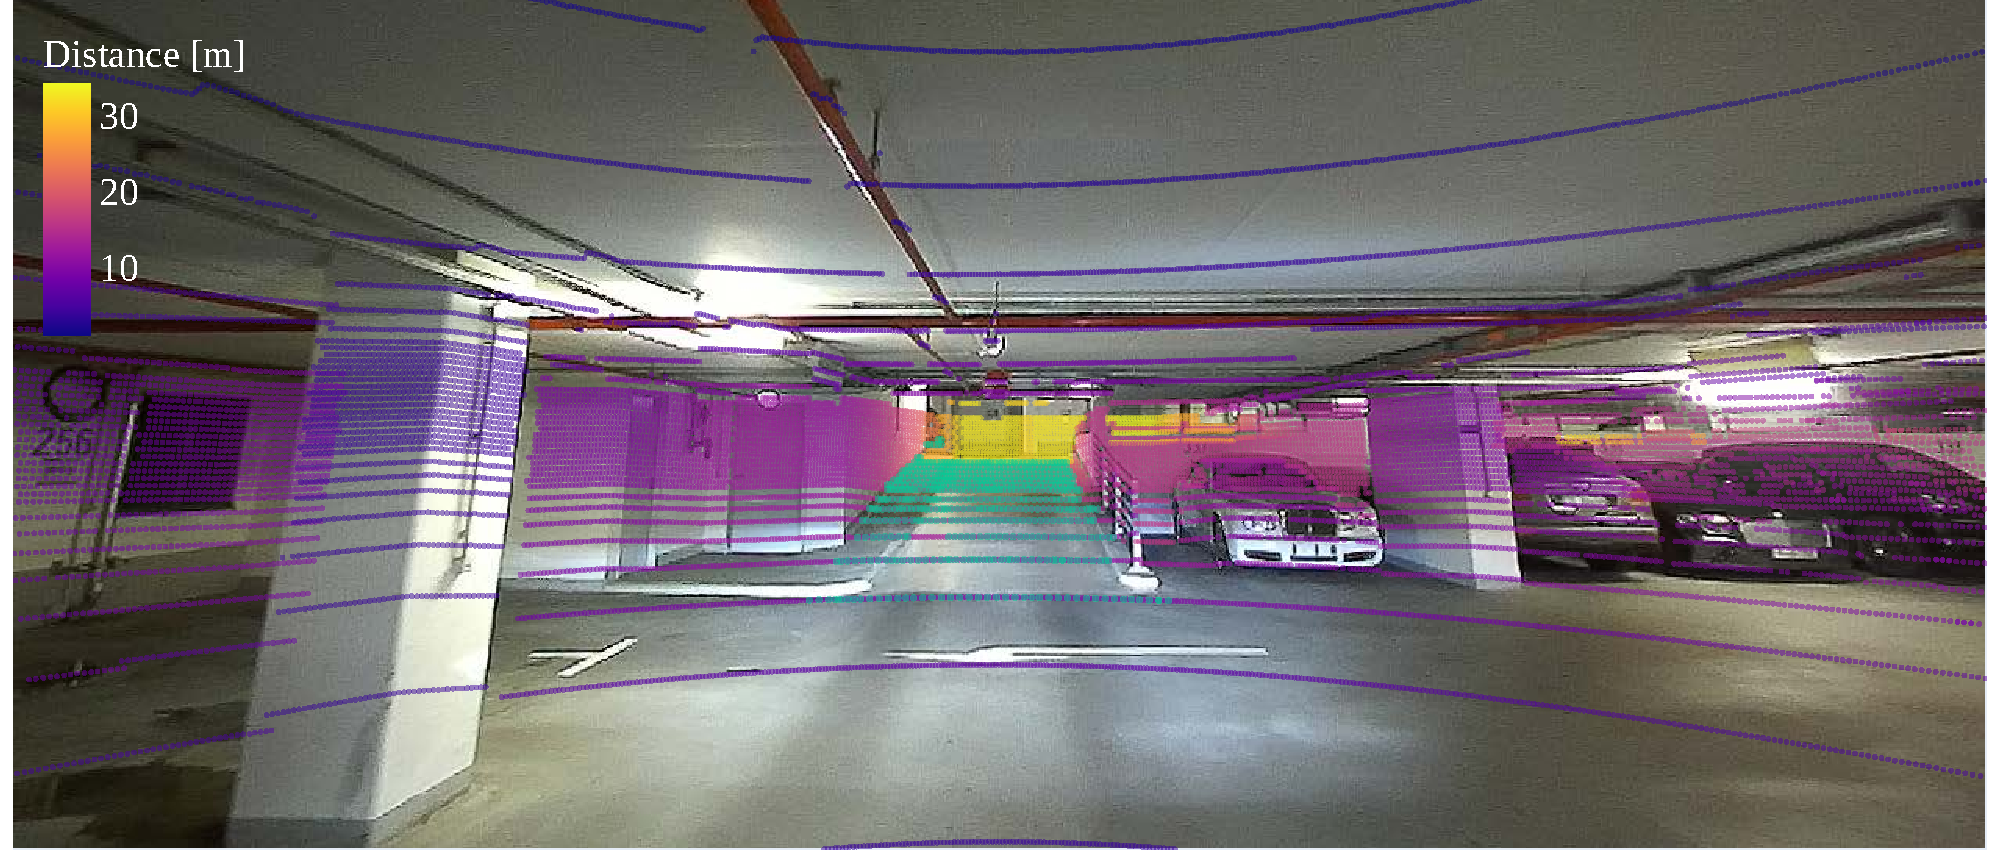
\includegraphics[width=1\linewidth]{points_projection.pdf}
    \caption{Ramp detection in action}
\end{figure}

\begin{figure}[htbp]
    \centering
    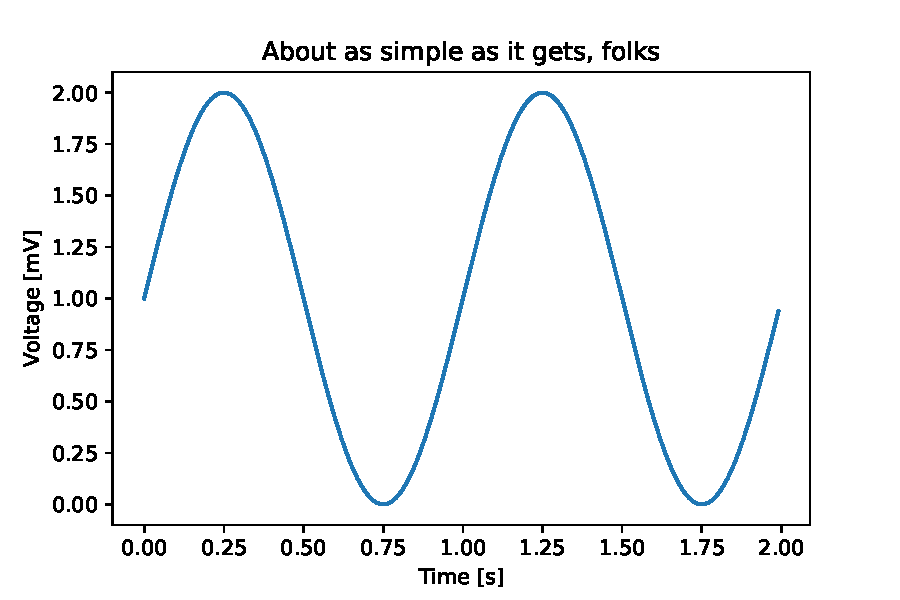
\includegraphics[width=0.7\linewidth]{matplotlib.pdf}
    \caption{Standard matplotlib}
\end{figure}

\begin{figure}[htbp]
    \centering
    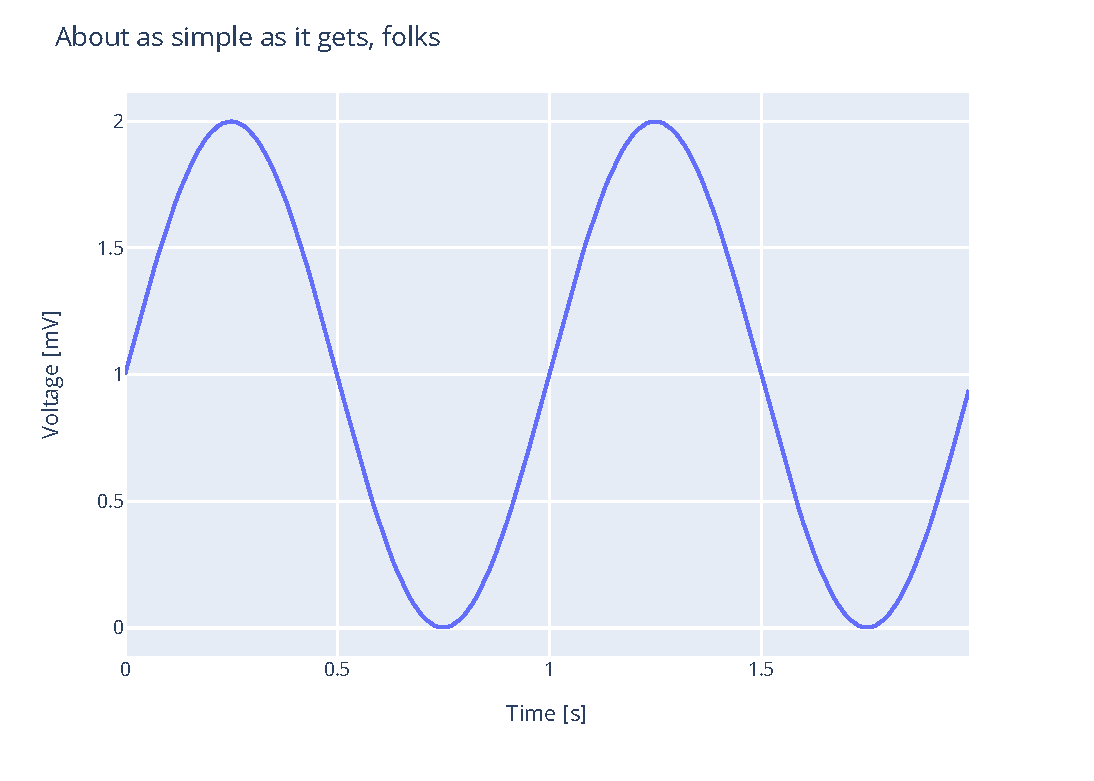
\includegraphics[width=0.7\linewidth]{plotly.pdf}
    \caption{Standard plotly}
\end{figure}